\begin{name}
	{\tenchude}{\tendethi}{LỚP TOÁN THẦY PHÁT}{\thoigian}
\end{name}
\setcounter{ex}{0}\setcounter{bt}{0}
\Opensolutionfile{ans}[ans/ans-2-TT-5-HongDuc-HCM-23]
\begin{ex}%[Đề thi thử tốt nghiệp THPT Quốc Gia năm 2023 - Trường THCS-THPT Hồng Đức - Thành phố Hồ Chí Minh]%[Ninh Tiến Nam - 2EX623]%[2H3Y2-4]
	Trong KG $Oxyz$, mặt phẳng $(P)\colon x+2y-5z-1=0$ đi qua điểm nào sau đây?
	\choice
	{$(1;2;-5)$}
	{$(2;1;1)$}
	{$(1;2;1)$}
	{\True $(4;1;1)$}
	\loigiai{Điểm có tọa độ $(4;1;1)$ thỏa mãn phương trình của $(P)$ nên thuộc mặt phẳng $(P)$. 
	}
\end{ex}

\begin{ex}%[Đề thi thử tốt nghiệp THPT Quốc Gia năm 2023 - Trường THCS-THPT Hồng Đức - Thành phố Hồ Chí Minh]%[Ninh Tiến Nam - 2EX623]%[2D1Y1-2]
	Cho hàm số $y=f(x)$ có bảng biến thiên như sau
\begin{center}

\begin{tikzpicture}	
		\tkzTabInit[nocadre=false,lgt=1.2,espcl=2.5,deltacl=0.6]	
		{$x$ /0.6,$f'(x)$ /0.6,$f(x)$/2}%phần bắt buộc	
		{$-\infty$, $2$, $3$,  $+\infty$}	
		\tkzTabLine{,+,$0$, -, $0$, +,}	
		\tkzTabVar{-/$-\infty$,+/$1$,-/$0$,+/$+\infty$}	
\end{tikzpicture}
\end{center}
Hàm số đã cho nghịch biến trên các khoảng nào dưới đây?
	\choice
	{$(3;+\infty)$}
	{$(-\infty;2)$}
	{$(-\infty;1)$}
	{\True $(2;3)$}
	\loigiai{
		Từ bảng biến thiên, ta suy ra hàm số đã cho nghịch biến trên $(2;3)$.
	}
\end{ex}

\begin{ex}%[Đề thi thử tốt nghiệp THPT Quốc Gia năm 2023 - Trường THCS-THPT Hồng Đức - Thành phố Hồ Chí Minh]%[Ninh Tiến Nam - 2EX623]%[2H1Y3-2]
Cho khối hộp chữ nhật có chiều dài bằng $4$, chiều rộng bằng $3$, chiều cao bằng $2$. Thể tích khối hộp đã cho bằng 	
	\choice
	{\True $24$}
	{$9$}
	{$14$}
	{$20$}
	\loigiai{Thể tích khối hộp chữ nhật bằng  $4\cdot 3\cdot 2=24$.
	}
\end{ex}

\begin{ex}%[Đề thi thử tốt nghiệp THPT Quốc Gia năm 2023 - Trường THCS-THPT Hồng Đức - Thành phố Hồ Chí Minh]%[Ninh Tiến Nam - 2EX623]%[2D1Y2-2]
	Cho hàm số $y=f(x)$ có bảng biến thiên như sau
\begin{center}

\begin{tikzpicture}	
		\tkzTabInit[nocadre=false,lgt=1.2,espcl=2.5,deltacl=0.6]	
		{$x$ /0.6,$f'(x)$ /0.6,$f(x)$/2}%phần bắt buộc	
		{$-\infty$, $-1$, $0$, $1$, $+\infty$}	
		\tkzTabLine{,+,$0$, -, $0$, +, $0$, -,}	
		\tkzTabVar{-/$-\infty$,+/$2$,-/$1$,+/$2$,-/$-\infty$}	
\end{tikzpicture}
\end{center}
Giá trị cực đại của hàm số đã cho bằng	
	\choice
	{$1$}
	{\True $2$}
	{$0$}
	{$-14$}
	\loigiai{Hàm số đã cho có giá trị cực đại bằng $2$.
	}
\end{ex}

\begin{ex}%[Đề thi thử tốt nghiệp THPT Quốc Gia năm 2023 - Trường THCS-THPT Hồng Đức - Thành phố Hồ Chí Minh]%[Ninh Tiến Nam - 2EX623]%[2D1Y3-1]
	Giá trị nhỏ nhất của hàm số $f(x)=x^4-6x^2+2$ trên đoạn $[-2;1]$ bằng
	\choice
	{$-6$}
	{$-3$}
	{ $2$}
	{\True $-7$}
	\loigiai{Ta có $f'(x)=4x^3-12x$; 
		$$f'(x)=0\Leftrightarrow \hoac{&x=0\in [-2;1]\\&x=\pm \sqrt{3}\in [-2;1].}$$
		Do $f(-2)=-6$, $f(-\sqrt{3})=f(\sqrt{3})=-7$, $f(0)=2$, $f(1)=-3$ nên giá trị nhỏ nhất của hàm số đã cho bằng $-7$.
	}
\end{ex}

\begin{ex}%[Đề thi thử tốt nghiệp THPT Quốc Gia năm 2023 - Trường THCS-THPT Hồng Đức - Thành phố Hồ Chí Minh]%[Ninh Tiến Nam - 2EX623]%[1D3Y4-3]
	Cho cấp số nhân  $\left(u_n \right) $ với $u_1=2$ và công bội $q=-3$. Số hạng $u_2$ của cấp số nhân đã cho bằng 
	\choice
	{\True $-6$}
	{$-\dfrac{2}{3}$}
	{$-1$}
	{$6$}
	\loigiai{Ta có $u_2=u_1\cdot q=2\cdot (-3)=-6$.
	}
\end{ex}

\begin{ex}%[Đề thi thử tốt nghiệp THPT Quốc Gia năm 2023 - Trường THCS-THPT Hồng Đức - Thành phố Hồ Chí Minh]%[Ninh Tiến Nam - 2EX623]%[2H3Y1-3]
	Trong KG $Oxyz$, cho mặt cầu $(S)\colon x^2+(y-3)^2+(z+3)^2=25$. Tọa độ tâm của mặt cầu đã cho là
	\choice
	{$(0;-3;-3)$}
	{$(0;-3;3)$}
	{$(0;3;3)$}
	{\True $(0;3;-3)$}
	\loigiai{Mặt cầu $(S)$ có tọa độ tâm là $(0;3;-3)$.
	}
\end{ex}

\begin{ex}%[Đề thi thử tốt nghiệp THPT Quốc Gia năm 2023 - Trường THCS-THPT Hồng Đức - Thành phố Hồ Chí Minh]%[Ninh Tiến Nam - 2EX623]%[2D1Y5-1]
\immini{Hàm số nào dưới đây có đồ thị dạng như đường cong hình vẽ
	bên?
	\choice
	{$y=-x^3+3x+1$}
	{$y=x^3+3x^2+1$}
	{$y=-x^4+2x^2$}
	{\True $y=-x^4+2x^2+1$}}{
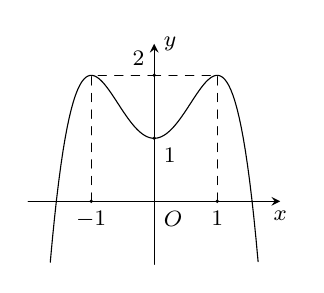
\begin{tikzpicture}[>=stealth,line join=round,line cap=round,font=\footnotesize,scale=.8]	
	\draw[->] (-2,0)--(2,0)node[below]{$x$};	
	\draw[->] (0,-1)--(0,2.5)node[right]{$y$};	
	\draw (0,0) node[below right] {$O$};			
	\fill (-1,0)circle(0.03)node[below]{$-1$}	
	(0,1)circle(0.03)node[below right]{$1$}	
	(1,0)circle(0.03)node[below]{$1$}	
	(0,2)circle(0.03)node[above left]{$2$}	;	
	\draw[ domain=-1.65:1.65, samples=100] plot (\x,{-(\x)^4+2*(\x)^2+1});	
	\draw[dashed] (-1,0)|-(0,2) (1,0)|-(0,2);	
\end{tikzpicture}}
	\loigiai{Đường cong ở hình vẽ bên có dạng đồ thị của hàm số trùng phương với hệ số $a<0$ và cắt trục tung tại điểm có tung độ $1$.\\
		Trong các đáp án chỉ có đồ thị của hàm số $y=-x^4+2x^2+1$  thỏa mãn.
	}
\end{ex}

\begin{ex}%[Đề thi thử tốt nghiệp THPT Quốc Gia năm 2023 - Trường THCS-THPT Hồng Đức - Thành phố Hồ Chí Minh]%[Ninh Tiến Nam - 2EX623]%[2H3Y3-3]
Trong KG $Oxyz$, đường thẳng $d\colon \heva{&x=2+t\\&y=4-2t\\&z=-3+3t}$	đi qua điểm nào dưới đây?
	\choice
	{$(1;-2;-3)$}
	{$(1;4;-3)$}
	{\True $(3;2;0)$}
	{$(4;2;0)$}
	\loigiai{Với $t=1$ thì $x=3$, $y=2$, $z=0$. Vậy đường thẳng $d$ đi qua $(3;2;0)$.
	}
\end{ex}

\begin{ex}%[Đề thi thử tốt nghiệp THPT Quốc Gia năm 2023 - Trường THCS-THPT Hồng Đức - Thành phố Hồ Chí Minh]%[Ninh Tiến Nam - 2EX623]%[2D2Y5-1]
	Nghiệm của phương trình $\log_5(x-1)=2$ là
	\choice
	{$x=11$}
	{$x=6$}
	{\True $x=26$}
	{$x=2$}
	\loigiai{Điều kiện $x-1>0$.\\
		Khi đó, 
		$\log_5(x-1)=2\Leftrightarrow x-1=5^2\Leftrightarrow x=26$.\\
	Vậy nghiệm của phương trình đã cho là $x=26$.
	}
\end{ex}

\begin{ex}%[Đề thi thử tốt nghiệp THPT Quốc Gia năm 2023 - Trường THCS-THPT Hồng Đức - Thành phố Hồ Chí Minh]%[Ninh Tiến Nam - 2EX623]%[1D2Y1-2]
	Nếu chọn $1$ nam và $1$ nữ làm trực nhật từ một tổ gồm $4$ nam và $6$ nữ thì có bao nhiêu cách?
	\choice
	{\True $24$}
	{$2$}
	{$10$}
	{$1$}
	\loigiai{
\begin{itemize}
			\item Số cách chọn $1$ bạn nam là $4$;
			\item Số cách chọn $1$ bạn nữ là $6$.
\end{itemize}
	Vậy số cách chọn là $4\cdot 6=24$.}
\end{ex}

\begin{ex}%[Đề thi thử tốt nghiệp THPT Quốc Gia năm 2023 - Trường THCS-THPT Hồng Đức - Thành phố Hồ Chí Minh]%[Ninh Tiến Nam - 2EX623]%[2D4Y1-1]
	Mô-đun của số phức $3i+1$ bằng
	\choice
	{$2$}
	{$4$}
	{$10$}
	{\True $\sqrt{10}$}
	\loigiai{Mô-đun của số phức $3i+1$ bằng $\sqrt{10}$.
	}
\end{ex}

\begin{ex}%[Đề thi thử tốt nghiệp THPT Quốc Gia năm 2023 - Trường THCS-THPT Hồng Đức - Thành phố Hồ Chí Minh]%[Ninh Tiến Nam - 2EX623]%[2D3Y2-1]
	Biết $\displaystyle\int\limits_{0}^{2}f(x)\mathrm{\,d}x=2$ và $\displaystyle\int\limits_{2}^{4}f(x)\mathrm{\,d}x=-5$, khi đó $\displaystyle\int\limits_{0}^{4}f(x)\mathrm{\,d}x$ bằng
	\choice
	{$3$}
	{$-10$}
	{\True $-3$}
	{$-7$}
	\loigiai{Ta có $\displaystyle\int\limits_{0}^{4}f(x)\mathrm{\,d}x=\displaystyle\int\limits_{0}^{2}f(x)\mathrm{\,d}x+\displaystyle\int\limits_{2}^{4}f(x)\mathrm{\,d}x=2+(-5)=-3$.
	}
\end{ex}

\begin{ex}%[Đề thi thử tốt nghiệp THPT Quốc Gia năm 2023 - Trường THCS-THPT Hồng Đức - Thành phố Hồ Chí Minh]%[Ninh Tiến Nam - 2EX623]%[2D1Y2-2]
Cho hàm số $f(x)$ có bảng xét dấu của $f'(x)$  như sau
\begin{center}

\begin{tikzpicture}	
	\tkzTabInit[nocadre=false,lgt=1.2,espcl=2.5,deltacl=0.6]	
	{$x$ /0.6,$f'(x)$ /0.6}%phần bắt buộc	
	{$-\infty$, $-2$, $-1$, $0$, $1$, $+\infty$}	
	\tkzTabLine{,+,$0$, +, $0$,-,$0$, +, $0$, -,}	
	%\tkzTabVar{-/$-\infty$,+/$3$,-/$-1$,+/$3$,-/$-\infty$}	
\end{tikzpicture}
\end{center}	
Số điểm cực trị của hàm số đã cho là
	\choice
	{$1$}
	{\True $3$}
	{$2$}
	{$0$}
	\loigiai{Hàm số $f'(x)$ đổi dấu khi qua các điểm $-1$, $0$, $1$ nên hàm số đã cho có $3$ điểm cực trị.
	}
\end{ex}

\begin{ex}%[Đề thi thử tốt nghiệp THPT Quốc Gia năm 2023 - Trường THCS-THPT Hồng Đức - Thành phố Hồ Chí Minh]%[Ninh Tiến Nam - 2EX623]%[2D2Y3-1]
Cho $a$ là số thực dương tùy ý, tính	$\log_5(5a)$.
	\choice
	{$5+a$}
	{$5+\log_5a$}
	{$1+a$}
	{\True $1+\log_5a$}
	\loigiai{Ta có $\log_5(5a)=1+\log_5a$.
	}
\end{ex}

\begin{ex}%[Đề thi thử tốt nghiệp THPT Quốc Gia năm 2023 - Trường THCS-THPT Hồng Đức - Thành phố Hồ Chí Minh]%[Ninh Tiến Nam - 2EX623]%[2H2Y1-2]
	Diện tích xung quanh của hình trụ có độ dài đường sinh $l$ và bán kính $r$ là
	\choice
	{$\dfrac{1}{3}\pi rl$}
	{$3\pi rl$}
	{\True $2\pi rl$}
	{$\pi rl$}
	\loigiai{Diện tích xung quanh của hình trụ có độ dài đường sinh $l$ và bán kính $r$ là $2\pi rl$.
	}
\end{ex}

\begin{ex}%[Đề thi thử tốt nghiệp THPT Quốc Gia năm 2023 - Trường THCS-THPT Hồng Đức - Thành phố Hồ Chí Minh]%[Ninh Tiến Nam - 2EX623]%[2H3Y1-1]
	Trong KG $Oxyz$, hình chiếu vuông góc của điểm $M(1;2;-1)$ trên mặt phẳng $(Oxz)$ có tọa	độ là
	\choice
	{$(1;2;0)$}
	{$(0;2;-1)$}
	{\True $(1;0;-1)$}
	{$(0;-2;0)$}
	\loigiai{Hình chiếu vuông góc của điểm $M(1;2;-1)$ trên mặt phẳng $(Oxz)$ có tọa	độ là $(1;0;-1)$.
	}
\end{ex}

\begin{ex}%[Đề thi thử tốt nghiệp THPT Quốc Gia năm 2023 - Trường THCS-THPT Hồng Đức - Thành phố Hồ Chí Minh]%[Ninh Tiến Nam - 2EX623]%[2D3Y1-1]
	Họ tất cả các nguyên hàm của hàm số $f(x)=-\sin x+4x$ là
	\choice
	{$-\cos x+4x^2+C$}
	{\True $\cos x+2x^2+C$}
	{$-\cos x+2x^2+C$}
	{$\cos x+4$}
	\loigiai{Ta có $\displaystyle\int\limits\left(-\sin x+4x \right)\mathrm{\,d}x=\cos x+2x^2+C $.
	}
\end{ex}

\begin{ex}%[Đề thi thử tốt nghiệp THPT Quốc Gia năm 2023 - Trường THCS-THPT Hồng Đức - Thành phố Hồ Chí Minh]%[Ninh Tiến Nam - 2EX623]%[2D3Y1-2]
Họ tất cả các nguyên hàm của hàm số $f(x)=\dfrac{2x+3}{x+1}$ trên khoảng $(-1;+\infty)$ là	
	\choice
	{$2x+\dfrac{1}{(x-1)^2}+C$}
	{\True $2x+\ln (x+1)+C$}
	{$2x+3\ln (x+1)+C$}
	{$2x-\dfrac{1}{(x+1)^2+C}$}
	\loigiai{Trên $(-1;+\infty)$, ta có $\displaystyle\int\limits\left(\dfrac{2x+3}{x+1}\right)\mathrm{\,d}x= \displaystyle\int\limits\left(2+\dfrac{1}{x+1}\right)\mathrm{\,d}x=2x+\ln (x+1)+C$.
	}
\end{ex}

\begin{ex}%[Đề thi thử tốt nghiệp THPT Quốc Gia năm 2023 - Trường THCS-THPT Hồng Đức - Thành phố Hồ Chí Minh]%[Ninh Tiến Nam - 2EX623]%[2D4Y2-2]
	Trên mặt phẳng toạ độ $Oxy$, điểm biểu diễn số phức $z=(2-i)^2$  là
	\choice
	{$M(-4;3)$}
	{\True $Q(3;-4)$}
	{$N(4;-3)$}
	{$P(-3;4)$}
	\loigiai{Điểm biểu diễn số phức $z=(2-i)^2=3-4i$ có tọa độ là $Q(3;-4)$.
	}
\end{ex}

\begin{ex}%[Đề thi thử tốt nghiệp THPT Quốc Gia năm 2023 - Trường THCS-THPT Hồng Đức - Thành phố Hồ Chí Minh]%[Ninh Tiến Nam - 2EX623]%[2H3Y1-2]
	Trong KG $Oxyz$, cho $\overrightarrow{a}=(3;1;-2)$ và $\overrightarrow{b}=(-2;0;-3)$. Tích vô hướng $\overrightarrow{a}\cdot \left( 2\overrightarrow{a}+\overrightarrow{b}\right) $.
	\choice
	{$29$}
	{$26$}
	{$25$}
	{\True $28$}
	\loigiai{Ta có $2\overrightarrow{a}+\overrightarrow{b}=(4;2;-7)$ nên
		$$\overrightarrow{a}\cdot \left( 2\overrightarrow{a}+\overrightarrow{b}\right) =3\cdot 4+1\cdot 2+(-2)\cdot (-7)=28.$$
	}
\end{ex}

\begin{ex}%[Đề thi thử tốt nghiệp THPT Quốc Gia năm 2023 - Trường THCS-THPT Hồng Đức - Thành phố Hồ Chí Minh]%[Ninh Tiến Nam - 2EX623]%[2H3Y3-1]
	Trong KG $Oxyz$, véc-tơ nào dưới đây là một véc-tơ chỉ phương của đường thẳng đi qua hai điểm $M(1;3;-1)$ và $N(3;5;1)$?
	\choice
	{\True $\overrightarrow{u}_4=(1;1;1)$}
	{$\overrightarrow{u}_1=(1;1;-1)$}
	{$\overrightarrow{u}_2=(4;8;0)$}
	{$\overrightarrow{u}_3=(2;4;0)$}
	\loigiai{Ta có $\overrightarrow{MN}=(2;2;2)$; ta thấy $\overrightarrow{u}_4=\dfrac{1}{2}\overrightarrow{MN}$ nên $\overrightarrow{u}_4$ là một véc-tơ chỉ phương của đường thẳng $MN$.
	}
\end{ex}

\begin{ex}%[Đề thi thử tốt nghiệp THPT Quốc Gia năm 2023 - Trường THCS-THPT Hồng Đức - Thành phố Hồ Chí Minh]%[Ninh Tiến Nam - 2EX623]%[2D1Y5-3]
Cho hàm số $y=f(x)$ có bảng biến thiên như sau
\begin{center}

\begin{tikzpicture}
	\tkzTabInit[nocadre=false,lgt=1.2,espcl=2.5,deltacl=0.6]
	{$x$ /0.6,$f'(x)$ /0.6,$f(x)$/2}%phần bắt buộc
	{$-\infty$, $0$, $3$,  $+\infty$}
	\tkzTabLine{,+,$0$, -, $0$, +,}
	\tkzTabVar{-/$-\infty$,+/$0$,-/$-1$,+/$+\infty$}
\end{tikzpicture}
\end{center}	
Số nghiệm thực của phương trình $2f(x)+3=0$ là
	\choice
	{$0$}
	{$3$}
	{$2$}
	{\True $1$}
	\loigiai{Ta có $2f(x)+3=0\Leftrightarrow f(x)=-\dfrac{3}{2}$, từ bảng biến thiên của hàm số $y=f(x)$ suy ra phương trình $2f(x)+3=0$ có $1$ nghiệm.
	}
\end{ex}

\begin{ex}%[Đề thi thử tốt nghiệp THPT Quốc Gia năm 2023 - Trường THCS-THPT Hồng Đức - Thành phố Hồ Chí Minh]%[Ninh Tiến Nam - 2EX623]%[2D2B3-2]
	Cho $a$ và $b$ là hai số thực dương thỏa mãn $3\log_2a=\log_4\left(a^2b \right)  $. Mệnh đề nào dưới đây đúng?
	\choice
	{$a^3=b$}
	{$a=b^2$}
	{\True $a^4=b$}
	{$a=b^4$}
	\loigiai{Ta có
\begin{eqnarray*}
	&&3\log_2a=\log_4\left(a^2b \right)\\&\Leftrightarrow& 3\log_2a=\dfrac{1}{2}\log_2\left( a^2b\right) \\&\Leftrightarrow& 6\log_2a=\log_2\left( a^2b\right)\\&\Leftrightarrow& \log_2a^6=\log_2\left( a^2b\right)
	\\&\Leftrightarrow& a^6=a^2b
	\\&\Leftrightarrow& a^4=b.
\end{eqnarray*}
	}
\end{ex}

\begin{ex}%[Đề thi thử tốt nghiệp THPT Quốc Gia năm 2023 - Trường THCS-THPT Hồng Đức - Thành phố Hồ Chí Minh]%[Ninh Tiến Nam - 2EX623]%[1H3B3-3]
	\immini{Cho hình chóp $S.ABCD$  có đáy $ABCD$ là hình thoi cạnh $a$, $SA$ vuông
		góc với mặt phẳng đáy, $SA=BD=a\sqrt{3}$. Góc giữa đường thẳng $SC$ và
		mặt phẳng $(ABCD)$ bằng
	\choice
	{\True $60^\circ$}
	{$30^\circ$}
	{$90^\circ$}
	{$45^\circ$}}{
\begin{tikzpicture}[>=stealth,line join=round,line cap=round,font=\footnotesize,scale=.7]	
	\def\a{3}	
	\def\b{1}	
	\path (0,0)coordinate (O) 	
	+(140:\b)coordinate (A)	
	(A)+(0:\a)coordinate (D) (A)+(90:\a)coordinate (S)	
	($(A)!2!(O)$)coordinate (C)	
	($(D)!2!(O)$)coordinate (B)	
	($(D)!.5!(C)$)coordinate (M);	
	\draw (S)--(B)--(C)--(D)--cycle (S)--(C);	
	\draw[dashed](S)--(A)--(D)--(B)--(A) ;	
	\foreach \x/\g in {S/90,A/150,B/210,C/-30,D/0} \fill (\x) circle (0.03)+(\g:3mm) node[scale=.9] {$\x$};		
\end{tikzpicture}}
	\loigiai{
	\immini{	Gọi $O$ là giao điểm của $AC$ và $BD$.\\	Ta có $AC=2AO=2\sqrt{AB^2-OB^2}=2\sqrt{a^2-\left( \dfrac{a\sqrt{3}}{2}\right)^2 }=a$.\\
		Do $SA\perp (ABCD)$ nên góc giữa đường thẳng $SC$ và
		mặt phẳng $(ABCD)$ bằng góc giữa đường thẳng $SC$ và đường thẳng $AC$.\\
		Do $\triangle SAC$ vuông tại $A$ nên $\widehat{SCA}<90^\circ$, suy ra $\left(SC,AC \right)=\widehat{SCA}$.\\
			Ta có $\tan \widehat{SCA}=\dfrac{SA}{AC}=\dfrac{a\sqrt{3}}{a}=\sqrt{3}$ nên $\widehat{SCA}=60^\circ$.}{
\begin{tikzpicture}[>=stealth,line join=round,line cap=round,font=\footnotesize,scale=.7]	
			\def\a{3}	
			\def\b{1}	
			\path (0,0)coordinate (O) 	
			+(140:\b)coordinate (A)	
			(A)+(0:\a)coordinate (D) (A)+(90:\a)coordinate (S)	
			($(A)!2!(O)$)coordinate (C)	
			($(D)!2!(O)$)coordinate (B)	
			($(D)!.5!(C)$)coordinate (M);	
			\draw (S)--(B)--(C)--(D)--cycle (S)--(C);	
			\draw[dashed](S)--(A)--(D)--(B)--(A)--(C) ;	
			\foreach \x/\g in {S/90,A/150,B/210,C/-30,D/0,O/-90} \fill (\x) circle (0.03)+(\g:3mm) node[scale=.9] {$\x$};		
\end{tikzpicture}}
	}
\end{ex}

\begin{ex}%[Đề thi thử tốt nghiệp THPT Quốc Gia năm 2023 - Trường THCS-THPT Hồng Đức - Thành phố Hồ Chí Minh]%[Ninh Tiến Nam - 2EX623]%[2H3B2-7]
Cắt mặt cầu tâm $I$ bởi mặt phẳng qua $I$, 	thiết diện thu được là hình tròn có diện tích bằng $9\pi$. Thể tích khối cầu đã cho bằng
	\choice
	{$12\pi$}
	{\True $36\pi$}
	{$18\pi$}
	{$27\pi$}
	\loigiai{\immini{Cắt mặt cầu tâm $I$ bởi mặt phẳng qua $I$, ta được hình tròn lớn bán kính $R$ bằng bán kính mặt cầu.\\
	Theo bài ra ta có $\pi R^2=9\pi\Rightarrow R=3$.\\
	Vậy thể tích khối cầu đã cho là $V=\dfrac{4}{3}\pi R^3=\dfrac{4}{3}\cdot \pi \cdot 3^3=36\pi$.	
	}{
\begin{tikzpicture}[>=stealth,line join=round,line cap=round,font=\footnotesize,scale=.5]
\def\R{2}
\def\b{.6}
\path (0,0)coordinate(O)
($({\R*cos (-20)},{\b*sin (-20)})$)coordinate(A)
;
\draw (O)circle(\R)
(O)+(0:\R) arc(0:-180:{\R} and {\b})
(O)--(A)node[midway,above,scale=.6]{$R$}
;
\draw[dashed](O)+(0:\R) arc(0:180:{\R} and {\b});
\end{tikzpicture}		
}
	}
\end{ex}

\begin{ex}%[Đề thi thử tốt nghiệp THPT Quốc Gia năm 2023 - Trường THCS-THPT Hồng Đức - Thành phố Hồ Chí Minh]%[Ninh Tiến Nam - 2EX623]%[2H1B3-1]
\immini{Cho hình lăng trụ đứng $ABCD.A'B'C'D'$ có đáy là hình chữ nhật cạnh	$BC=a$, $BD=2BC$ và  $AA'=2\sqrt{3}a$. Diện tích toàn phần của  hình lăng trụ đã cho bằng
	\choice
	{$16a^2\sqrt{3}$}
	{$14a^2\left(1+\sqrt{3} \right) $}
	{\True $6a^2\left(2+\sqrt{3} \right) $}
	{$24a^2$}}{	
\begin{tikzpicture}[>=stealth,line join=round,line cap=round,font=\footnotesize,scale=.7]
	\def\a{3}	
	\def\b{2}	
	\def\c{3}	
	\def\goc{-90}
	\path (0,0)coordinate (A')	
	+(0:\a)coordinate (B')	
	+(50:\b)coordinate (D')
	($(D')+(B')-(A')$)coordinate (C')	
	(B')	+(\goc:\c)coordinate (B)	
	(A')	+(\goc:\c)coordinate (A)	
	(C')		+(\goc:\c)coordinate (C)
	(D')		+(\goc:\c)coordinate (D);
	\draw (A')--(B')--(C')--(D')--cycle (A')--(A)--(B)--(C)--(C') (B)--(B');
	\draw[dashed](A)--(D)--(C) (D')--(D)--(B);
	\foreach \x/\g in {A'/180,B'/0,C'/0,D'/150,A/180,B/0,C/0,D/150} \fill (\x) circle (0.03)+(\g:3mm) node[scale=.9] {$\x$};
		\draw pic[draw,angle radius=2mm] {right angle = B--C--D}; 
\end{tikzpicture}}	
	\loigiai{
		Tam giác $BDC$ vuông tại $C$ nên $CD=\sqrt{BD^2-BC^2}=\sqrt{3}BC=\sqrt{3}a$.\\
		Diện tích xung quanh khối hình hộp chữ nhật là 
		$$S_{\text{xq}}=2(BC+CD)\cdot AA'=2\left( a+\sqrt{3}a\right) \cdot 2\sqrt{3}a=\left(4\sqrt{3}+12 \right)a^2. $$
		Diện tích một đáy của hình hộp chữ nhật là
		$$S_{\text{đáy}}=BC\cdot CD= a\cdot \sqrt{3}a=\sqrt{3}a^2.$$ 
Vậy diện tích toàn phần của hình hộp chữ nhật là
$$S_{\text{tp}}=S_{xq}+2S_{\text{đáy}}=\left(4\sqrt{3}+12 \right)a^2+2\sqrt{3}a^2=\left(\sqrt{3}+2 \right)6a^2.$$
	}
\end{ex}

\begin{ex}%[Đề thi thử tốt nghiệp THPT Quốc Gia năm 2023 - Trường THCS-THPT Hồng Đức - Thành phố Hồ Chí Minh]%[Ninh Tiến Nam - 2EX623]%[2D1B4-1]
	Gọi $y=y_0$, $x=x_0$ là các đường tiệm cận ngang và tiệm cận đứng của đồ thị hàm số $y=\dfrac{2x^2+5x+2}{(x+2)^2}$, khi đó tổng $x_0+y_0$ bằng
	\choice
	{\True $0$}
	{$\dfrac{5}{2}$}
	{$-\dfrac{5}{2}$}
	{$-4$}
	\loigiai{Hàm số đã cho xác định trên $\mathscr{D}=\mathbb{R}\setminus\{-2\}$.\\
		Ta có $y=\dfrac{2x^2+5x+2}{(x+2)^2}=\dfrac{(x+2)\left(2x+1 \right) }{(x+2)^2}=\dfrac{2x+1}{x+2}$.\\
		Do đó, đồ thị hàm số đã cho có tiệm cận ngang là $y=2$ và tiệm cận đứng là $x=-2$.\\
		Vậy $x_0+y_0=(-2)+2=0$.
	}
\end{ex}

\begin{ex}%[Đề thi thử tốt nghiệp THPT Quốc Gia năm 2023 - Trường THCS-THPT Hồng Đức - Thành phố Hồ Chí Minh]%[Ninh Tiến Nam - 2EX623]%[2D2B6-1]
	Tập nghiệm của bất phương trình $6^{2x+1}\ge6^{x^2-3x+7}$ là
	\choice
	{$[1;6]$}
	{\True $[2;3]$}
	{$[1;5]$}
	{$(-\infty;1]\cup [6;+\infty)$}
	\loigiai{Ta có 
\begin{eqnarray*}
		6^{2x+1}\ge6^{x^2-3x+7}\Leftrightarrow 2x+1\ge x^2-3x+7\Leftrightarrow x^2-5x+6\le 0\Leftrightarrow 2\le x\le 3.
\end{eqnarray*}
	Vậy tập nghiệm của bất phương trình đã cho là $S=[2;3]$
	}
\end{ex}

\begin{ex}%[Đề thi thử tốt nghiệp THPT Quốc Gia năm 2023 - Trường THCS-THPT Hồng Đức - Thành phố Hồ Chí Minh]%[Ninh Tiến Nam - 2EX623]%[2D3B3-1]
\immini{Diện tích S của phần gạch sọc trong hình được tính bằng
	\choice
{$\displaystyle\int\limits_{-3}^{1}\left| -x^2-2x-3\right| \mathrm{\,d}x$}
{$\displaystyle\int\limits_{-3}^{1}\left(  x^2-2x-3\right)\mathrm{\,d}x  $}
{$\displaystyle\int\limits_{-3}^{1}\left(  x^2+2x-3\right) \mathrm{\,d}x $}
{\True $\displaystyle\int\limits_{-3}^{1}\left(  -x^2-2x+3\right) \mathrm{\,d}x $}}{
\begin{tikzpicture}[>=stealth,line join=round,line cap=round,font=\footnotesize,scale=.6]
\draw[->] (-3.5,0)--(3,0)node[below]{$x$};
\draw[->] (0,-2.4)--(0,4.5)node[right]{$y$};
\draw (0,0) node[below right] {$O$};			
\fill (-3,0)circle(0.03)node[below]{$-3$}
(1,0)circle(0.03)node[below]{$1$};
\draw[ domain=-3.1:2.1, samples=100] plot (\x,{(\x)^2+\x-2});
\draw[ domain=-3.4:2.5, samples=100] plot (\x,{-(\x)+1});
\draw[dashed] (-3,0)|-(0,4) ;
\fill
[pattern=dots, domain=-3:1, samples=100] plot (\x,{(\x)^2+\x-2})	--plot (\x,{-(\x)+1})
;
\draw (2.2,3)node[rotate=-100,scale=.7]{$f(x)=x^2+x-2$}
(2,-2)node[scale=.7]{$g(x)=-x+1$}
;
\end{tikzpicture}}
\loigiai{
Diện tích hình phẳng giới hạn bởi đồ thị hàm số $f(x)$ và $g(x)$ là
$$S=\displaystyle\int\limits_{-3}^{1}\left| (-x+1)-\left( x^2+x-2\right) \right| \mathrm{\,d}x=\displaystyle\int\limits_{-3}^{1}\left(  (-x+1)-\left( x^2+x-2\right) \right)  \mathrm{\,d}x=\displaystyle\int\limits_{-3}^{1}\left(   -x^2-2x+3\right)   \mathrm{\,d}x.$$
}
\end{ex}

\begin{ex}%[Đề thi thử tốt nghiệp THPT Quốc Gia năm 2023 - Trường THCS-THPT Hồng Đức - Thành phố Hồ Chí Minh]%[Ninh Tiến Nam - 2EX623]%[2D4B2-2]
Cho hai số phức $z_1=-3+2i$ và $z_2=1-i$. Phần ảo của số phức $\overline{z_1}+z_2$ bằng	
	\choice
	{\True $-3$}
	{$3$}
	{$3i$}
	{$-2$}
	\loigiai{
		Ta có $\overline{z_1}+z_2=(-3-2i)+(1-i)=-2-3i$.\\
		Vậy phần ảo của số phức $\overline{z_1}+z_2$ bằng	$-3$.
			}
\end{ex}

\begin{ex}%[Đề thi thử tốt nghiệp THPT Quốc Gia năm 2023 - Trường THCS-THPT Hồng Đức - Thành phố Hồ Chí Minh]%[Ninh Tiến Nam - 2EX623]%[2D2B4-5]
Biết rằng vi khuẩn E.coli là vi khuẩn gây tiêu chảy đường ruột, gây đau bụng dữ dội, ngoài ra cứ sau $20$ phút thì số lượng vi khuẩn tăng gấp đôi, nghĩa là số lượng tính theo công thức $S=S_0\cdot 2^n$, $S_0$ là số lượng ban đầu, $n$ là số lần nhân đôi. Ban đầu chỉ có $40$ con vi khuẩn nói trên trong đường ruột, hỏi sau bao
lâu số lượng vi khuẩn là $671\,088\,640$ con?	
	\choice
	{$24$ giờ}
	{\True $8$ giờ}
	{$12$ giờ}
	{$48$ giờ}
	\loigiai{
		Nếu $S_0=40$; $S=671\,088\,640$ thì số lần nhân đôi là $n=\log_2\left(\dfrac{S}{S_0} \right)= \log_2\left(\dfrac{671\,088\,640}{40} \right)=24$.\\
		Vậy thời gian từ lúc đầu đến lúc số lượng vi khuẩn là $671\,088\,640$ con là
		$$20\cdot 24=480\ (\text{phút})=8\ (\text{giờ}).$$	
	}
\end{ex}

\begin{ex}%[Đề thi thử tốt nghiệp THPT Quốc Gia năm 2023 - Trường THCS-THPT Hồng Đức - Thành phố Hồ Chí Minh]%[Ninh Tiến Nam - 2EX623]%[2H3B2-7]
	Trong KG $Oxyz$, mặt phẳng $(P) $ đi qua $M(1;1;-1)$ và song song với mặt phẳng $(Q)\colon 2x+3y+z-9=0$ có phương trình là
	\choice
	{$x+y-2z=0$}
	{\True $2x+3y+z-4=0$}
	{$2x-y+z=0$}
	{$2x+3y+z+3=0$}
	\loigiai{Mặt phẳng $(P)$ song song với mặt phẳng $(Q)\colon 2x+3y+z-9=0$ nên có véc-tơ pháp tuyến là $(2;3;1)$.\\
		Ta có $M(1;1;-1)\in (P)$ nên phương trình $(P)$ là
		$$2(x-1)+3(y-1)+(z+1)=0\Leftrightarrow 2x+3y+z-4=0.$$
	}
\end{ex}

\begin{ex}%[Đề thi thử tốt nghiệp THPT Quốc Gia năm 2023 - Trường THCS-THPT Hồng Đức - Thành phố Hồ Chí Minh]%[Ninh Tiến Nam - 2EX623]%[2D1B2-1]
	Cho hàm số $y=4x^3-6x^2+5$. Tìm giá trị cực tiểu của hàm số đã cho.
	\choice
	{\True $y_{\text{CT}}=3$}
	{$y_{\text{CT}}=1$}
	{$y_{\text{CT}}=0$}
	{$y_{\text{CT}}=5$}
	\loigiai{
		Ta có $y'=12x^2-12x$; $y''=24x-12$; $y'=0\Leftrightarrow 12x^2-12x=0\Leftrightarrow x=0$ hoặc $x=1$.\\
		Do $y''(0)=-12<0$, $y''(1)=12>0$ nên hàm số đạt cực tiểu tại $x=1$ và  $y_{\text{CT}}=3$.
			}
\end{ex}

\begin{ex}%[Đề thi thử tốt nghiệp THPT Quốc Gia năm 2023 - Trường THCS-THPT Hồng Đức - Thành phố Hồ Chí Minh]%[Ninh Tiến Nam - 2EX623]%[2H3B1-3]
	Trong KG $Oxyz$, phương trình mặt cầu có tâm $I(0;2;0)$ và đi qua $M(2;0;0)$ có phương trình là
	\choice
	{$(x-2)^2+y^2+z^2=2\sqrt{2}$}
	{\True $x^2+(y-2)^2+z^2=8$}
	{$(x-2)^2+y^2+z^2=8$}
	{$x^2+(y-2)^2+z^2=2\sqrt{2}$}
	\loigiai{
		Ta có $IM=\sqrt{(2-0)^2+(0-2)^2+(0-0)^2}=2\sqrt{2}$.\\
		Vậy phương trình mặt cầu là
		$x^2+(y-2)^2+z^2=8$.
	}
\end{ex}

\begin{ex}%[Đề thi thử tốt nghiệp THPT Quốc Gia năm 2023 - Trường THCS-THPT Hồng Đức - Thành phố Hồ Chí Minh]%[Ninh Tiến Nam - 2EX623]%[2D1B1-3]
	Cho hàm số $f(x)=\dfrac{mx-4}{x-m}$ ($m$ là tham số thực). Có bao nhiêu giá trị nguyên $m$ thuộc $(-6;6)$ để hàm số đã cho nghịch biến trên $(0;+\infty)$?
	\choice
	{\True $3$}
	{$2$}
	{$4$}
	{$5$}
	\loigiai{Hàm số xác định khi $x\ne m$.\\
		Ta có $f'(x)=\dfrac{-m^2+4}{(x-m)^2}$, hàm số đã cho nghịch biến trên $(0;+\infty)$ khi và chỉ khi
		$$\heva{&m\le 0\\&-m^2+4<0}\Leftrightarrow m<-2.$$
		Vậy có $3$ tất cả các giá trị nguyên $m$ thuộc $(-6;6)$ để hàm số đã cho nghịch biến trên $(0;+\infty)$ là $m\in \{-5,-4,-3\}$.
			}
\end{ex}

\begin{ex}%[Đề thi thử tốt nghiệp THPT Quốc Gia năm 2023 - Trường THCS-THPT Hồng Đức - Thành phố Hồ Chí Minh]%[Ninh Tiến Nam - 2EX623]%[2D2K5-5]
Cho phương trình $4^{x+1}+4^{1-x}-(m+1)\left(2^{x+1}-2^{2-x} \right) 	+8m-16=0$ ($m$ là tham số thực). Tìm tất cả các giá trị của tham số $m$ để phương trình đã cho có nghiệm trên đoạn $[0;1]$.
	\choice
	{$\left[0;\dfrac{3}{2} \right]$ }
	{$\left[1;\dfrac{5}{2} \right)$ }
	{$\left[\dfrac{3}{2};+\infty \right) $}
	{\True $\left[1;\dfrac{5}{2} \right] $}
	\loigiai{
		Ta có 
\begin{eqnarray*}
		&&4^{x+1}+4^{1-x}-(m+1)\left(2^{2+x}-2^{2-x} \right) 	+8m-16=0\\
		&\Leftrightarrow& \left(4^{x+1}-8+4^{1-x} \right)  -2(m+1)\left(2^{1+x}-2^{1-x}\right) +8m-8=0\\
		&\Leftrightarrow&\left( 2^{x+1}-2^{1-x}\right)^2 -2(m+1)\left(2^{1+x}-2^{1-x}\right) +8m-8=0\\
		&\Leftrightarrow& \left(2^{x+1}-2^{1-x}-4 \right) \left( 2^{x+1}-2^{1-x}-2m+2\right)=0\\
	&\Leftrightarrow& 	\hoac{&2^{x+1}-2^{1-x}-4=0\ (1)\\&2^{x+1}-2^{1-x}-2m+2=0\ (2).}
\end{eqnarray*} 
\begin{itemize}
		\item Xét $(1)$. Đặt $t=2^x$, ($t>0$), phương trình $(1)$ trở  thành
		$$2t-\dfrac{2}{t}-4=0\Leftrightarrow 2t^2-4t-2=0\Leftrightarrow \hoac{&t=1+\sqrt{2}\\&t=1-\sqrt{2}\ (\text{loại}).}$$
		Với $t=1+\sqrt{2}$, suy ra $x=\log_2\left(1+\sqrt{2} \right)>1 $.
\item Xét $(2)$. $2^{x+1}-2^{1-x}-2m+2=0$.\\
Xét hàm số $y=f(x)=2^{x+1}-2^{1-x}-2m+2$ trên $[0;1]$, $f'(x)=\left( 2^{x+1}+2^{1-x}\right)\ln 2>0 $.\\
Bảng biến thiên của hàm số như sau
\begin{center}

\begin{tikzpicture}
	\tkzTabInit[nocadre=false,lgt=1.2,espcl=2.5,deltacl=0.8]
	{$x$ /0.6,$f'(x)$ /0.6,$f(x)$/2}%phần bắt buộc
	{$0$,$1$ }
	\tkzTabLine{,+,}
	\tkzTabVar{-/$-2m+2$,+/$5-2m$}
\end{tikzpicture}
\end{center}
Vậy phương trình đã cho có nghiệm trên $[0;1]$ khi và chỉ khi 
$$-2m+2\le 0 \le 5-2m\Leftrightarrow 1\le m\le \dfrac{5}{2}.$$
\end{itemize}
	}
\end{ex}

\begin{ex}%[Đề thi thử tốt nghiệp THPT Quốc Gia năm 2023 - Trường THCS-THPT Hồng Đức - Thành phố Hồ Chí Minh]%[Ninh Tiến Nam - 2EX623]%[2H2K1-2]
Cho hình trụ có chiều cao bằng $2\sqrt{5}$. Cắt hình trụ đã cho bởi mặt phẳng song song với trục, cách trục một khoảng $\sqrt{5}$, thiết diện thu được là hình vuông. Diện tích xung quanh hình trụ đã cho bằng	
	\choice
	{$8\pi\sqrt{10}$}
	{$4\pi\sqrt{10}$}
	{$10\pi\sqrt{5}$}
	{\True $20\pi\sqrt{2}$}
	\loigiai{\immini{Giả sử $OO'$ là trục của hình trụ.\\
	Gọi   $H$ là hình chiếu của $O$ trên $MN$, trong đó $MNPQ$ là thiết diện cho trong giả thiết bài toán.	$MNPQ$ là hình vuông nên $MN=MQ=2\sqrt{5}$.\\
		Tam giác vuông $ONH$ có $OH=\sqrt{5}$, $NH=\dfrac{1}{2}MN=\dfrac{1}{2}\cdot 2\sqrt{5}=\sqrt{5}$ nên
		$$ON=\sqrt{OH^2+NH^2}=\sqrt{\left( \sqrt{5}\right)^2+\left( \sqrt{5}\right)^2 }=\sqrt{10}.$$
		Vậy diện tích xung quanh hình trụ là
		$S_{\text{xq}}=2\pi \cdot \sqrt{10}\cdot 2\sqrt{5}=20\pi\sqrt{2}$.
	}{
\begin{tikzpicture}[>=stealth,line join=round,line cap=round,font=\footnotesize,scale=.9]
			\def\a{2}
			\def\b{.48}
			\def\h{3}
			\path (0,0)coordinate (O)
			+(90:\h)coordinate (O')	
			+(0:\a)coordinate (B)	
			+(180:\a)coordinate (A)
			($({\a*cos(-80)},{\b*sin(-80)})$)coordinate (M)+(90:\h)coordinate(Q)
				($({\a*cos(50)},{\b*sin(50)})$)coordinate (N)+(90:\h)coordinate(P)
		($(M)!.5!(N)$)coordinate(H)	;	
			\draw 	(A)arc(-180:0: {\a} and {\b}) (A)--+(90:\h)(B)--+(90:\h)
			(O')ellipse ({\a} and {\b})	
			(P)--(Q)--(M);
			\draw[dashed]  	(A)arc(180:0: {\a} and {\b})
			(M)--(N)--(P)
		(N)--(O)--(H) (O)--(O')			;
				\draw pic[draw,angle radius=2mm] {right angle = O--H--N}; 
			\foreach \x/\g in {A/180,B/0,O/180,M/-90,N/40,P/90,Q/90,H/0,O'/90} \fill (\x) circle (0.03)+(\g:3mm) node[scale=.9] {$\x$};
\end{tikzpicture}}
		}
\end{ex}

\begin{ex}%[Đề thi thử tốt nghiệp THPT Quốc Gia năm 2023 - Trường THCS-THPT Hồng Đức - Thành phố Hồ Chí Minh]%[Ninh Tiến Nam - 2EX623]%[2D3K2-2]
	Cho hàm số $f(x)$, biết 	$f(1)=1$, $f'(x)=\dfrac{2x}{3x+1-\sqrt{3x+1}}$, $x>0$. Khi đó, $\displaystyle\int\limits_{1}^{5}f(x)\mathrm{\,d}x$ bằng 
	\choice
	{$\dfrac{128}{9}$}
	{$\dfrac{184}{9}$}
	{$\dfrac{440}{27}$}
	{\True $\dfrac{916}{81}$}
	\loigiai{
		Xét $\displaystyle\int\dfrac{2x}{3x+1-\sqrt{3x+1}}\mathrm{\,d}x$ với $x>0$.\\
		 Đặt $t=\sqrt{3x+1}\Rightarrow x=\dfrac{t^2-1}{3}$, ta có  $\dfrac{2t}{3}\mathrm{\,d}t=\mathrm{d}x$.\\
		 Do đó
\begin{eqnarray*}
		 \displaystyle\int\dfrac{2x}{3x+1-\sqrt{3x+1}}\mathrm{\,d}x&=& \displaystyle\int\dfrac{2\cdot \frac{t^2-1}{3}}{t^2-t}\cdot\dfrac{2t}{3}\mathrm{\,d}t
		 \\&=&\dfrac{4}{9}\displaystyle\int\dfrac{\left( t^2-1\right)t }{t^2-t}\mathrm{\,d}t=\dfrac{4}{9}\displaystyle\int\left(t+1 \right) \mathrm{\,d}t=\dfrac{2}{9}t^2+\dfrac{4}{9}t+C\\&=&\dfrac{2}{9}(3x+1)+\dfrac{4}{9}\sqrt{3x+1}+C.
\end{eqnarray*}
	Do 	đó $f(x)=\dfrac{2}{9}(3x+1)+\dfrac{4}{9}\sqrt{3x+1}+C_1$, mà $f(1)=1$ nên $C_1=-\dfrac{7}{9}$. Suy ra $f(x)=\dfrac{2}{9}(3x+1)+\dfrac{4}{9}\sqrt{3x+1}-\dfrac{7}{9}$.\\
	Vậy 
\begin{eqnarray*}
	\displaystyle\int\limits_{1}^{5}f(x)\mathrm{\,d}x&=&\displaystyle\int\limits_{1}^{5}\left(\dfrac{2}{9}(3x+1)+\dfrac{4}{9}\sqrt{3x+1}-\dfrac{7}{9} \right) \mathrm{\,d}x\\
	&=&\dfrac{2}{9}\displaystyle\int\limits_{1}^{5}\left(3x+1 \right) \mathrm{\,d}x+\dfrac{4}{9}\displaystyle\int\limits_{1}^{5}\sqrt{3x+1}\mathrm{\,d}x-\dfrac{7}{9}\displaystyle\int\limits_{1}^{5}\mathrm{\,d}x.
\end{eqnarray*}
Ta có $\dfrac{2}{9}\displaystyle\int\limits_{1}^{5}\left(3x+1 \right) \mathrm{\,d}x=\dfrac{2}{9}\cdot \left(\dfrac{3}{2}x^2 +x\right) \Bigg|_1^5=\dfrac{80}{9}$.\\
Xét $\dfrac{4}{9}\displaystyle\int\limits_{1}^{5}\sqrt{3x+1}\mathrm{\,d}x$.\\
 Đặt $t=\sqrt{3x+1}$, ta có $\dfrac{2t}{3}\mathrm{\,d}t=\mathrm{d}x$, $x=1$ thì $t=2$, $x=5$ thì $t=4$, suy ra
$$\dfrac{4}{9}\displaystyle\int\limits_{1}^{5}\sqrt{3x+1}\mathrm{\,d}x=\dfrac{4}{9}\displaystyle\int\limits_{2}^{4}\dfrac{2t^2}{3} \mathrm{\,d}t=\dfrac{4}{9}\cdot \left( \dfrac{2t^3}{9}\right)\Bigg|_2^4=\dfrac{448}{81}.$$
Ta có $\dfrac{7}{9}\displaystyle\int\limits_{1}^{5}\mathrm{\,d}x=\dfrac{7}{9}x\big|_1^5=\dfrac{28}{9}$.\\
Vậy $\displaystyle\int\limits_{1}^{5}f(x)\mathrm{\,d}x=\dfrac{80}{9}+\dfrac{448}{81}-\dfrac{28}{9}=\dfrac{916}{81}$.
	}
\end{ex}

\begin{ex}%[Đề thi thử tốt nghiệp THPT Quốc Gia năm 2023 - Trường THCS-THPT Hồng Đức - Thành phố Hồ Chí Minh]%[Ninh Tiến Nam - 2EX623]%[2D3K1-1]
Cho hàm số $f(x)$ liên tục trên $(0;+\infty)$. Biết $\ln 2x$ là một nguyên hàm của hàm số $f(x)\mathrm{e}^x$. Họ tất cả các nguyên hàm của hàm số $f'(x)\mathrm{e}^x$ là	
	\choice
	{\True $\dfrac{1}{x}-\ln 2x+C$}
{$\dfrac{1}{x}-\dfrac{1}{2}\ln 2x+C$}
	{$\dfrac{2}{x}+\ln 2x+C$}
	{$\dfrac{1}{2x}-\ln 2x+C$}
	\loigiai{
	Trên $(0;+\infty)$,	ta có $(\ln 2x)'=\dfrac{2}{2x}=\dfrac{1}{x}$ nên	$f(x)\mathrm{e}^x=\dfrac{1}{x}\Rightarrow f(x)=\dfrac{1}{x\mathrm{e}^x}\Rightarrow f'(x)=-\dfrac{1}{x^2\mathrm{e}^x}-\dfrac{1}{x\mathrm{e}^x}$.\\
	Vậy $\displaystyle\int f'(x)\mathrm{e}^x\mathrm{\,d}x=\displaystyle\int\left(-\dfrac{1}{x^2}-\dfrac{1}{x} \right)\mathrm{\,d}x=\dfrac{1}{x}-\ln x +C_1=\dfrac{1}{x}-\ln 2x+C_1+\ln 2=\dfrac{1}{x}-\ln 2x+C $.
	}
\end{ex}

\begin{ex}%[Đề thi thử tốt nghiệp THPT Quốc Gia năm 2023 - Trường THCS-THPT Hồng Đức - Thành phố Hồ Chí Minh]%[Ninh Tiến Nam - 2EX623]%[1H3K5-4]
\immini{	Cho hình chóp $S.ABCD$  có đáy là hình thang cạnh
	$AB=2a$, $AD=DC=CB=a$, $SA=3a$ và $SA$ vuông góc với mặt phẳng
	đáy. Khoảng cách giữa hai đường thẳng $AC$ và $SB$ bằng
	\choice
	{$\dfrac{3a}{2}$}
	{\True $\dfrac{3a\sqrt{10}}{10}$}
	{$\dfrac{3a\sqrt{10}}{20}$}
	{$\dfrac{3a}{4}$}}{
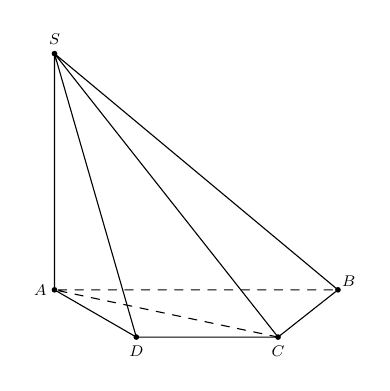
\begin{tikzpicture}[>=stealth,line join=round,line cap=round,font=\footnotesize,scale=.6]
	\path
	(0,0)coordinate (A)
	+(90:5)coordinate (S)
	+ (0:6)coordinate (B)
	++ (-30:2)coordinate (D)
	+ (0:3)coordinate (C)
		;
	\draw (S)--(A)--(D)--(C)--(B)--cycle (S)--(C) (D)--(S);
	\draw[dashed] (C)--(A)--(B);
	\foreach \x/\g in {S/90,A/180,B/40,C/-90,D/-90} \fill (\x) circle (0.06)+(\g:3mm) node[scale=.7] {$\x$};
\end{tikzpicture}	}
	\loigiai{\immini{Gọi $M$ là trung điểm của $AB$, hình thang $AMCD$ ($AM\parallel CD$) có $AM=CD$ nên là hình bình hành, suy ra $MC=AD=a=\dfrac{1}{2}AB$. Do đó, tam giác $ACB$ vuông tại $C$.\\
		Dựng hình chữ nhật $ACBI$, gọi $H$ là hình chiếu của $A$ trên $SI$.\\
		Ta có $BI\perp AI$, $BI\perp SA$ nên $BI\perp AH$. Do $AH\perp SI$, $AH\perp BI$ nên $AH\perp (SIB)$.\\
		Ta có $AC\parallel IB$ nên $AC\parallel (SBI)$ suy ra 
		$$\mathrm{d}(AC,SB)=\mathrm{d}(AC,(SBI))=\mathrm{d}(A,(SBI))=AH.$$	
			}{
\begin{tikzpicture}[>=stealth,line join=round,line cap=round,font=\footnotesize,scale=.6]
			\path
			(0,0)coordinate (A)
			(90:6)coordinate (S)
			 (2,-2)coordinate (D)
		 (6,-2)coordinate (C)
		 ($(A)+2*(C)-2*(D)$)coordinate (B)
			($(A)!.5!(B)$)coordinate (M)
			($(B)+(A)-(C)$)coordinate (I)
			($(S)!.6!(I)$)coordinate (H)
			;
			\draw (S)--(A)--(D)--(C)--(B)--cycle (S)--(C) (S)--(B) (S)--(D) ;
			\draw[dashed] (I)--(C)--(A)--(B) (S)--(I)--(A)--(H) (I)--(B);
			\draw pic[draw,angle radius=2mm] {right angle = A--I--B}
			pic[draw,angle radius=2mm] {right angle = A--H--I}
			pic[draw,angle radius=2mm] {right angle = A--C--B}
			; 
			\foreach \x/\g in {S/90,A/180,B/40,C/-90,D/-90,M/-90,I/70,H/0} \fill (\x) circle (0.05)+(\g:3mm) node[scale=.7] {$\x$};
\end{tikzpicture}}
\noindent 	Xét tam giác vuông $SIA$, ta có $SA=3a$, $AI=BC=a$ nên $AH=\dfrac{SA\cdot AI}{\sqrt{SA^2+AI^2}}=\dfrac{3a\cdot a}{\sqrt{(3a)^2+a^2}}=\dfrac{3a\sqrt{10}}{10}$.\\
Vậy 	khoảng cách giữa hai đường thẳng $AC$ và $SB$ bằng	$\dfrac{3a\sqrt{10}}{10}$.		
	}
\end{ex}

\begin{ex}%[Đề thi thử tốt nghiệp THPT Quốc Gia năm 2023 - Trường THCS-THPT Hồng Đức - Thành phố Hồ Chí Minh]%[Ninh Tiến Nam - 2EX623]%[2D2K3-2]
	Gọi $x$, $y$ là các số thực dương thỏa mãn $\log_9x=\log_6y=\log_4\left( \dfrac{x+y}{6}\right) $. Tính tỉ số $\dfrac{x}{y}$.
	\choice
	{$5$}
	{\True $4$}
	{$2$}
	{$3$}
	\loigiai{Đặt $\log_9x=\log_6y=\log_4\left( \dfrac{x+y}{6}\right)=t$, suy ra 
\begin{eqnarray*}
	\heva{&x=9^t\\&y=6^t\\&\dfrac{x+y}{6}=4^t}\Rightarrow \heva{&x=9^t\\&y=6^t\\&x+y=6\cdot 4^t}\Rightarrow 9^t+6^t=6\cdot 4^t\Rightarrow \left( \dfrac{3}{2}\right) ^{2t}+\left( \dfrac{3}{2}\right) ^{t}-6=0\Rightarrow \hoac{&\left( \dfrac{3}{2}\right) ^{t}=2\\&\left( \dfrac{3}{2}\right) ^{t}=-3\ (\text{loại}).}
\end{eqnarray*}
		Vậy $\dfrac{x}{y}=\left( \dfrac{9}{6}\right) ^{t}=\left( \dfrac{3}{2}\right) ^{2t}=4$.
	}
\end{ex}

\begin{ex}%[Đề thi thử tốt nghiệp THPT Quốc Gia năm 2023 - Trường THCS-THPT Hồng Đức - Thành phố Hồ Chí Minh]%[Ninh Tiến Nam - 2EX623]%[2D1K3-1]
	Gọi $S$ là tập giá trị của tham số $m$ để giá trị nhỏ nhất của hàm số $f(x)=\left|x^2-4x+m \right| $ trên $[1;4]$ bằng $6$. Tổng các phần tử của $S$ bằng 
	\choice
	{$6$}
	{$-10$}
	{\True $4$}
	{$-4$}
	\loigiai{Xét hàm số $y=g(x)=x^2-4x+m$ trên $[1;4]$, hàm số có bảng biến  thiên như sau
\begin{center}

\begin{tikzpicture}
			\tkzTabInit[nocadre=false,lgt=1.2,espcl=2.5,deltacl=0.6]
			{$x$ /0.6,$g'(x)$ /0.6,$g(x)$/2}%phần bắt buộc
			{$1$, $2$, $4$}
			\tkzTabLine{,-,$0$, +,}
			\tkzTabVar{+/$m-3$,-/$m-4$,+/$m$}
\end{tikzpicture}
\end{center}
		Do đó $\displaystyle\min_{[1;4]}f(x)=\displaystyle\min_{[1;4]}\left\lbrace|m-4|;|m| \right\rbrace $.
\begin{enumerate}[TH 1.]
			\item $\displaystyle\min_{[1;4]}\left\lbrace|m-4|;|m| \right\rbrace=|m-4|=6\Leftrightarrow \heva{&|m-4|=6\\&|m|\ge 6}\Leftrightarrow \heva{&\hoac{&m=-2\\&m=10}\\&|m|\ge 6}\Leftrightarrow m=10$.
			\item $\displaystyle\min_{[1;4]}\left\lbrace|m-4|;|m| \right\rbrace=|m|=6\Leftrightarrow \heva{&|m|=6\\&|m-4|\ge 6}\Leftrightarrow \heva{&\hoac{&m=-6\\&m=6}\\&|m-4|\ge 6}\Leftrightarrow m=-6$.
\end{enumerate}
Vậy $S=\{10;-6\}$, suy ra tổng các phần tử của $S$ bằng $10+(-6)=4$.	}
\end{ex}

\begin{ex}%[Đề thi thử tốt nghiệp THPT Quốc Gia năm 2023 - Trường THCS-THPT Hồng Đức - Thành phố Hồ Chí Minh]%[Ninh Tiến Nam - 2EX623]%[1D2K5-2]
	Trong một đợt phong trào \lq\lq  Thanh niên tình nguyện\rq\rq\ có $5$ học sinh khối $12$, $4$ học sinh khối $11$, và
	$3$ học sinh khối $10$, được chia làm nhiệm vụ ở $4$ thôn khác nhau $M$, $N$, $P$, $Q$ (Mỗi thôn $3$ học sinh). Tính xác	suất để thôn nào cũng có học sinh khối $12$ và học sinh khối $11$.
	\choice
	{\True $\dfrac{36}{385}$}
	{$\dfrac{144}{385}$}
	{$\dfrac{72}{385}$}
	{$\dfrac{18}{385}$}
	\loigiai{
		Gọi $\Omega$ là tập hợp tất cả các cách chọn  $3$ sinh viên tình nguyện ở mỗi thôn, ta có $n(\Omega)=\mathrm{C}_{12}^3\cdot \mathrm{C}_{9}^3\cdot \mathrm{C}_{6}^3\cdot \mathrm{C}_{3}^3$.\\
		Gọi $A$ là biến cố \lq\lq  Thôn nào cũng có học sinh khối $12$ và khối $11$ \rq\rq.\\
		Ta xét  khả năng thuận lợi cho biến cố $A$: Một thôn có $2$ học sinh lớp $12$, $1$ học sinh lớp $11$, ba thôn còn lại mỗi thôn có $1$ học sinh lớp $12$, $1$ học sinh lớp $11$, $1$ học sinh lớp $10$.\\
		Vậy các khả năng thuận lợi cho biến cố $A$ là $\left( \mathrm{C}_5^2\cdot \mathrm{C}_4^1\right) \cdot\left(  \mathrm{C}_3^1\cdot\mathrm{C}_3^1\cdot\mathrm{C}_3^1\right)\cdot \left(  \mathrm{C}_2^1\cdot\mathrm{C}_2^1\cdot\mathrm{C}_2^1\right)\cdot \left(  \mathrm{C}_1^1\cdot\mathrm{C}_1^1\cdot\mathrm{C}_1^1\right)\cdot 4  $ (nhân với $4$ vì có $4$ cách chọn một thôn có $2$ học sinh lớp $12$).\\
	Vậy xác suất của biến cố $A$ là
	$$\mathrm{P}(A)=\dfrac{\left( \mathrm{C}_5^2\cdot \mathrm{C}_4^1\right) \cdot\left(  \mathrm{C}_3^1\cdot\mathrm{C}_3^1\cdot\mathrm{C}_3^1\right)\cdot \left(  \mathrm{C}_2^1\cdot\mathrm{C}_2^1\cdot\mathrm{C}_2^1\right)\cdot \left(  \mathrm{C}_1^1\cdot\mathrm{C}_1^1\cdot\mathrm{C}_1^1\right)\cdot 4}{\mathrm{C}_{12}^3\cdot \mathrm{C}_{9}^3\cdot \mathrm{C}_{6}^3\cdot \mathrm{C}_{3}^3}=\dfrac{36}{385}.$$
	}
\end{ex}

\begin{ex}%[Đề thi thử tốt nghiệp THPT Quốc Gia năm 2023 - Trường THCS-THPT Hồng Đức - Thành phố Hồ Chí Minh]%[Ninh Tiến Nam - 2EX623]%[2D1K5-3]
	Cho hàm số có bảng biến thiên như sau
\begin{center}

\begin{tikzpicture}
		\tkzTabInit[nocadre=false,lgt=1.2,espcl=2.5,deltacl=0.6]
		{$x$ /0.6,$f'(x)$ /0.6,$f(x)$/2}%phần bắt buộc
		{$-\infty$, $-1$, $0$, $1$, $+\infty$}
		\tkzTabLine{,-,$0$, +, $0$, -, $0$, +,}
		\tkzTabVar{+/$+\infty$,-/$-2$,+/$-1$,-/$-2$,+/$+\infty$}
\end{tikzpicture}
\end{center}
Số nghiệm thuộc đoạn $[-\pi;2\pi]$ của phương trình $4f(\cos2x)+5=0$ là 
	\choice
	{\True $12$}
	{$9$}
	{$6$}
	{$10$}
	\loigiai{
	Với $x\in[-\pi;2\pi] $ thì $2x\in [-2\pi;4\pi]$,	ta có
	$$4f(\cos2x)+5=0\Leftrightarrow f(\cos2x)=-\dfrac{5}{4}\in (-2;-1).$$
	Kết hợp bảng biến thiên của $f(x)$, suy ra phương trình 	$f(\cos2x)=-\dfrac{5}{4}$ có $2$  nghiệm $\cos2x$ phân biệt trên $(-1;1)$. Ứng với mỗi giá trị của $\cos2x$ ta được $6$ giá trị  của $2x$ trên $2x\in [-2\pi;4\pi]$, tương ứng với $6$ giá trị của $x$.\\
	Vậy phương trình đã cho có $12$ nghiệm.
	}
\end{ex}

\begin{ex}%[Đề thi thử tốt nghiệp THPT Quốc Gia năm 2023 - Trường THCS-THPT Hồng Đức - Thành phố Hồ Chí Minh]%[Ninh Tiến Nam - 2EX623]%[2D1K1-2]
	\immini{Cho hàm số $f(x)$ có đồ thị $f'(x)$ như hình bên. Hàm số $g(x)=f(2-x)-\dfrac{1}{2}x^2+x$ nghịch biến trên khoảng nào dưới đây?
	\choice
	{$(-3;1)$}
 {	\True$(1;3)$}
	{$(0;1)$}
	{$(-1;1)$}}{
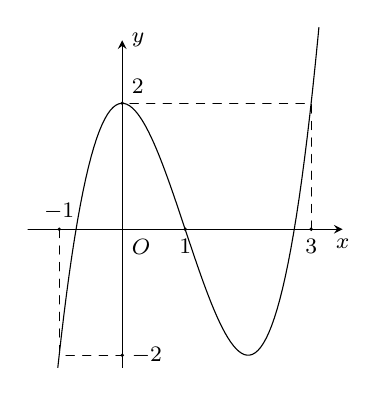
\begin{tikzpicture}[>=stealth,line join=round,line cap=round,font=\footnotesize,scale=.8]
\clip
(-1.5,-2.2)rectangle (3.7,3.2)
;
	\draw[->] (-1.5,0)--(3.5,0)node[below]{$x$};
	\draw[->] (0,-2.2)--(0,3)node[right]{$y$};
	\draw (0,0) node[below right] {$O$};			
	\fill (-1,0)circle(0.03)node[above]{$-1$}
	(0,-2)circle(0.03)node[right]{$-2$}
	(1,0)circle(0.03)node[below]{$1$}
	(3,0)circle(0.03)node[below]{$3$}
	(0,2)circle(0.03)node[above right]{$2$};
	\draw[ domain=-1.1:3.2, samples=100] plot (\x,{(\x)^3-3*(\x)^2+2});
	\draw[dashed] (-1,0)|-(0,-2) (3,0)|-(0,2);
\end{tikzpicture}}
	\loigiai{
	Ta có $g'(x)=-f'(2-x)-x+1=-f'(2-x)+(2-x)-1$, $g'(x)<0\Leftrightarrow (2-x)-1<f'(2-x)$.\\
	 Biểu diễn đồ thị hàm số $y=f'(t)$ và $y=t-1$ trên cùng một hệ trục tọa độ
\begin{center}
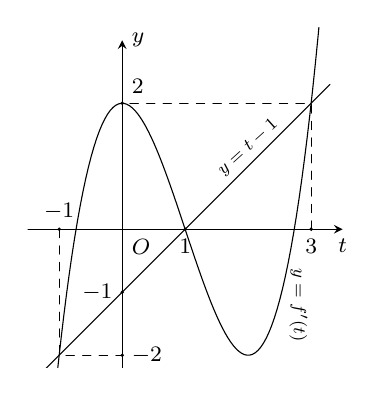
\begin{tikzpicture}[>=stealth,line join=round,line cap=round,font=\footnotesize,scale=.8]
	 \clip	 (-1.5,-2.2)rectangle (3.7,3.2)	 ;
	 \draw[->] (-1.5,0)--(3.5,0)node[below]{$t$};
	 \draw[->] (0,-2.2)--(0,3)node[right]{$y$};
	 \draw (0,0) node[below right] {$O$};			
	 \fill (-1,0)circle(0.03)node[above]{$-1$}
	 (0,-2)circle(0.03)node[right]{$-2$}
	 (0,-1)circle(0.03)node[left]{$-1$}
	 (1,0)circle(0.03)node[below]{$1$}
	 (3,0)circle(0.03)node[below]{$3$}
	 (0,2)circle(0.03)node[above right]{$2$};
	 \draw[ domain=-1.1:3.2, samples=100] plot (\x,{(\x)^3-3*(\x)^2+2});
	 \draw[ domain=-1.5:3.3, samples=100] plot (\x,{(\x)-1});
	 \draw[dashed] (-1,0)|-(0,-2) (3,0)|-(0,2);
	 \draw (2.8,-1.2)node[rotate=-90,scale=.8]{$y=f'(t)$}
(2,1.3)node[rotate=42,scale=.8]{$y=t-1$}
	 ;
\end{tikzpicture}	
\end{center}
		Ta có với $-1<2-x<1\Leftrightarrow 1<x<3$ thì $(2-x)-1<f'(2-x)$.\\
		Vậy hàm số $g(x)$ nghịch biến trên $(1;3)$.
	}
\end{ex}

\begin{ex}%[Đề thi thử tốt nghiệp THPT Quốc Gia năm 2023 - Trường THCS-THPT Hồng Đức - Thành phố Hồ Chí Minh]%[Ninh Tiến Nam - 2EX623]%[2D2K5-5]
Có bao nhiêu cặp số nguyên  $(x;y)$ thỏa mãn $\log_2(2x-2002)+x=y+1002+2^y$ và $1002\le x\le 2022$?	
	\choice
	{\True $10$}
	{$11$}
	{$12$}
	{$18$}
	\loigiai{Điều kiện $x>1001$.\\
	Ta có $\log_2(2x-2002)+x=y+1002+2^y
	\Leftrightarrow	\log_2(x-1001)+(x-1001)=\log_2\left(2^y \right) +2^y$.\\
Xét hàm số $y=\log_2t+t$ trên $(0;+\infty)$, ta có $y'=\dfrac{1}{t\ln 2}+1>0$ trên $(0;+\infty)$ nên hàm số $y=\log_2t+t$ đồng biến trên $(0;+\infty)$.\\
Do đó phương trình $\log_2(x-1001)+(x-1001)=\log_2\left(2^y \right) +2^y$ tương đương với $x-1001=2^y$.\\
Mà $1002\le x\le 2022$ suy ra $1<2^y<1021$, hay $0\le y<9{,}996$, lại có $y$ nguyên nên 	
$y\in \{0;1;2;\ldots;9\}$.\\
Thử lại với mỗi giá trị $y\in \{0;1;2;\ldots;9\}$, tương ứng ta tìm được $1$ giá trị nguyên của $x$.\\
Vậy có $10$ cặp số nguyên  $(x;y)$ thỏa mãn phương trình đã cho.
	}
\end{ex}

\begin{ex}%[Đề thi thử tốt nghiệp THPT Quốc Gia năm 2023 - Trường THCS-THPT Hồng Đức - Thành phố Hồ Chí Minh]%[Ninh Tiến Nam - 2EX623]%[1H3K4-3]
	Cho tam giác $ABC$ có $BC=a$, $\widehat{BAC}=135^\circ$. Trên đường thẳng vuông góc với mặt phẳng $(ABC)$ tại $A$ lấy điểm $S$ sao cho $SA=a\sqrt{2}$. Hình chiếu vuông góc  của $A$ trên $SB$, $SC$ lần lượt tại $M$, $N$. Số đo góc giữa hai mặt phẳng $(ABC)$ và $(AMN)$ bằng
	\choice
	{\True $45^\circ$}
	{$60^\circ$}
	{$75^\circ$}
	{$30^\circ$}
	\loigiai{
		\immini{
	Giả sử $AD$	là đường kính đường tròn ngoại tiếp tam giác $ABC$.\\
	Do $DC\perp SA $, $DC\perp AC$ nên $DC\perp (SAC)$, suy ra $DC\perp AN$, mà $AN\perp SC$, do đó $AN\perp SD$.\\
	Chứng minh tương tự ta cũng có $AM\perp SD$.\\
	Vậy $SD\perp (AMN)$.\\
	Ta có $SA\perp (ABC)$, $SD\perp (AMN)$ nên góc giữa $(ABC)$ và $(AMN)$ là góc giữa $SA$ và $SD$.\\
	Do $(O)$ ngoại tiếp  $\triangle ABC$ nên $AD=\dfrac{BC}{\sin A}=\dfrac{a}{\sin 135^\circ}=a\sqrt{2}$.
}{
\begin{tikzpicture}[>=stealth,line join=round,line cap=round,font=\footnotesize,scale=1]
			\def\a{3}
			\def\b{1}
			\def\h{3}
			\path (0,0)coordinate (O)
			+(0:\a)coordinate (D)	
			+(180:\a)coordinate (A)
			($({\a*cos(-120)},{\b*sin(-120)})$)coordinate (B)
			($({\a*cos(100)},{\b*sin(100)})$)coordinate (C)
			(A)+(90:\h)coordinate (S)
			($(S)!.4!(B)$)coordinate (M)($(S)!.6!(C)$)coordinate (N)
			;	
			\draw 	(A)arc(-180:0: {\a} and {\b}) (S)--(A)--(B)--(D)--cycle	  (S)--(B)	 (A)--(M)
		;
			\draw[dashed]  	(A)arc(180:0: {\a} and {\b})
				(A)--(C)--(B)(S)--(C)--(D)--(A)	(A)--(N)--(M);
			\draw pic[draw,angle radius=2mm] {right angle = A--B--D}
			 pic[draw,angle radius=2mm] {right angle = A--C--D}
			  pic[draw,angle radius=2mm] {right angle = A--M--B}
			  pic[draw,angle radius=2mm] {right angle = A--N--S}
			; 
			\foreach \x/\g in {A/180,B/-90,O/-90,C/90,D/40,S/90,M/180,N/20} \fill (\x) circle (0.03)+(\g:3mm) node[scale=.9] {\x};
\end{tikzpicture}
			}\noindent 	Xét tam giác vuông $SAD$, ta có $\tan\widehat{ASD}=\dfrac{AD}{SA}=\dfrac{a\sqrt{2}}{a\sqrt{2}}=1$ nên $\widehat{ASD}=1$.\\
		Vậy góc giữa $(ABC)$ và $(AMN)$ có số đo là $45^\circ$.
		}
\end{ex}

\begin{ex}%[Đề thi thử tốt nghiệp THPT Quốc Gia năm 2023 - Trường THCS-THPT Hồng Đức - Thành phố Hồ Chí Minh]%[Ninh Tiến Nam - 2EX623]%[2D1K2-2]
\immini{	Cho hàm số bậc  bốn $y=f(x)$ có đồ thị như hình vẽ. Số điểm cực trị của hàm số $g(x)=f\left(x^3-3x^2 \right) $ là
	\choice
	{$5$}
	{$9$}
	{\True $7$}
	{$3$}}{
\begin{tikzpicture}[>=stealth,line join=round,line cap=round,font=\footnotesize,scale=.7]
\clip
 (-6.5,-2.2)rectangle (4.2,2.7)
;
	\draw[->] (-6.5,0)--(4,0)node[below]{$x$};
	\draw[->] (0,-2.2)--(0,2.5)node[right]{$y$};
	\draw (0,0) node[above right] {$O$};			
	\fill	(-4,0)circle(0.03)node[below right]{$-4$}
;
	\draw (-6,2)..controls +(274:6) and +(245:2)..(-4,0)..controls+(66:9) and +(249:11)..(4,2);
\end{tikzpicture}}
	\loigiai{
	Ta có $g'(x)=\left(3x^2-6x \right)f'\left(x^3-3x^2 \right) $;
	$$g'(x)=0\Leftrightarrow \hoac{&3x^2-6x =0\\&f'\left(x^3-3x^2 \right)=0.}$$	
\begin{itemize}
	\item $3x^2-6x =0\Leftrightarrow x=0$ hoặc $x=2$.
	\item Từ đồ thị hàm số $y=f(x)$ suy ra phương trình $f'\left(x^3-3x^2 \right)=0$ tương đương với
	$$\hoac{&x^3-3x^2=a\ (a<-4)\\&x^3-3x^2=b\ (-4<b<0)\\&x^3-3x^2=c\ (c>0).}$$
	Xét hàm số $y=x^3-3x^2$, ta có $y'=3x^2-6x$, $y'=0\Leftrightarrow x=0$ hoặc $x=2$.\\Bảng biến thiên của hàm số như sau
\begin{center}

\begin{tikzpicture}
		\tkzTabInit[nocadre=false,lgt=1.2,espcl=2.5,deltacl=0.6]
		{$x$ /0.6,$y'$ /0.6,$y$/2}%phần bắt buộc
		{$-\infty$,  $0$, $2$, $+\infty$}
		\tkzTabLine{,+,$0$, -, $0$, +,}
		\tkzTabVar{-/$-\infty$,+/$0$,-/$-4$,+/$+\infty$}
\end{tikzpicture}
\end{center}
Từ bảng biến thiên của hàm số $y=x^3-3x^2$ suy ra phương trình $x^3-3x^2=a$ có $1$ nghiệm $x_1$ ($x_1<0$); $x^3-3x^2=b$ có $3$ nghiệm đơn phân biệt $x_2$, $x_3$, $x_4$ ($x_2<0<x_3<2<x_4$); $x^3-3x^2=c$ có $1$ nghiệm $x_5$ ($x_5>2$).
\end{itemize}
Vậy phương trình $g'(x)$ có $7$ nghiệm đơn phân biệt nên hàm số $g(x)$ có $7$ điểm cực trị.
	}
\end{ex}

\begin{ex}%[Đề thi thử tốt nghiệp THPT Quốc Gia năm 2023 - Trường THCS-THPT Hồng Đức - Thành phố Hồ Chí Minh]%[Ninh Tiến Nam - 2EX623]%[2D3G2-4]
	Cho hàm số $f(x)$ liên tục trên $\mathbb{R}$ sao cho $xf\left(x^3 \right)+f\left( 1-x^2\right)=-x^8+2x^5-3x  $, $\forall x\in \mathbb{R}$. Khi đó, tích phân $\displaystyle\int\limits_{-1}^{0}f(x)\mathrm{\,d}x$ bằng
	\choice
	{$\dfrac{579}{175}$}
	{$\dfrac{17}{10}$}
	{$-\dfrac{13}{6}$}
	{\True $-\dfrac{579}{175}$}
	\loigiai{ Giả sử $F(x)$ là một nguyên hàm của $f(x)$.\\
		Với mọi $x$, ta có
\begin{eqnarray*}
		&&xf\left(x^3 \right)+f\left( 1-x^2\right)=-x^8+2x^5-3x\\
		&\Rightarrow & x^2f\left(x^3 \right)+xf\left( 1-x^2\right)=-x^9+2x^6-3x^2.
\end{eqnarray*}
		Suy ra 
\begin{eqnarray*}
	\heva{&	\displaystyle\int\limits_{-1}^0\left( x^2f\left(x^3 \right)+xf\left( 1-x^2\right)\right)\mathrm{\,d}x =\displaystyle\int\limits_{-1}^0\left( -x^9+2x^6-3x^2\right)\mathrm{\,d}x=-\dfrac{43}{70}\\&	\displaystyle\int\limits_{0}^1\left( x^2f\left(x^3 \right)+xf\left( 1-x^2\right)\right)\mathrm{\,d}x =\displaystyle\int\limits_{0}^1\left(-x^9+2x^6-3x^2\right)\mathrm{\,d}x=-\dfrac{57}{70}.}
\end{eqnarray*}
	Ta có 	
\begin{eqnarray*}
	&&\displaystyle\int\left(x^2f\left(x^3 \right) \right)\mathrm{\,d}x =\dfrac{1}{3}\displaystyle\int f\left(x^3 \right)\mathrm{\,d}\left(x^3 \right) =\dfrac{1}{3}F\left(x^3 \right)+C_1,\\
	&&\displaystyle\int xf\left( 1-x^2\right) \mathrm{\,d}x=-\dfrac{1}{2}\displaystyle\int f\left( 1-x^2\right)\mathrm{\,d} \left(1-x^2 \right)=-\dfrac{1}{2}F\left( 1-x^2\right)+C_2 .
\end{eqnarray*}
	Do đó,
	$$\heva{&	\displaystyle\int\limits_{-1}^0\left( x^2f\left(x^3 \right)+xf\left( 1-x^2\right)\right)\mathrm{\,d}x =\dfrac{1}{3}\left[F(0)-F(-1) \right]-\dfrac{1}{2}\left[F(1)-F(0)\right]  \\&	\displaystyle\int\limits_{0}^1\left( x^2f\left(x^3 \right)+xf\left( 1-x^2\right)\right)\mathrm{\,d}x =\dfrac{1}{3}\left[F(1)-F(0) \right]-\dfrac{1}{2}\left[F(0)-F(1)\right]=\dfrac{5}{6}\left[F(1)-F(0)\right].}$$
	Suy ra
	$$\heva{&\dfrac{1}{3}\left[F(0)-F(-1) \right]-\dfrac{1}{2}\left[F(1)-F(0)\right]=-\dfrac{43}{70}\\&\dfrac{5}{6}\left[F(1)-F(0)\right]=-\dfrac{57}{70}}\Rightarrow F(0)-F(-1)=-\dfrac{579}{175}.$$
Vậy $\displaystyle\int\limits_{-1}^{0}f(x)\mathrm{\,d}x=F(0)-F(-1)=-\dfrac{579}{175}$.	}
\end{ex}

\Closesolutionfile{ans}
\begin{indapan}{10}
	{ans/ans-2-TT-5-HongDuc-HCM-23}
\end{indapan}